\documentclass[]{article}
\usepackage[frenchb]{babel}
\usepackage[T1]{fontenc}
\usepackage{textcomp}
\usepackage[utf8]{inputenc}
\usepackage{lmodern}
\usepackage{natbib}
\usepackage{multicol}
%pour liens hypertexte
\usepackage{hyperref}
\newcommand{\mhref}[3][blue]{\href{#2}{\color{#1}{#3}}}%

\usepackage{geometry}
%\geometry{verbose,tmargin=2cm,bmargin=2cm,lmargin=2cm,rmargin=2cm}

%% The amssymb package provides various useful mathematical symbols
\usepackage{amssymb}

% Pour les tables de matières
%\usepackage{shorttoc}

%pour les tableaux
\usepackage{tabularx}
\usepackage{multirow}
\usepackage{array}
\usepackage{ctable}
\usepackage{bm}
\newcolumntype{M}[1]{>{\arraybackslash}m{#1}}

%% The amsthm package provides extended theorem environments
\usepackage{amsthm}
\usepackage{numprint}

\graphicspath{{../Figures/}}

%%Pour les algorithmes
\usepackage{algorithmic}
\usepackage{algorithm}
\usepackage{natbib}
\usepackage{bibentry}

%% Variables locales
\newcommand{\SNOT}{{SNO~Tourbières }}
\def\adresseMO{https://forge-osuc.cnrs-orleans.fr/projects/sie-sno-tourbiere/repository/revisions/master/entry/Documentation/Modes_operatoires/}
\def\adressedocsmetier{https://forge-osuc.cnrs-orleans.fr/projects/sie-sno-tourbiere/repository/revisions/master/entry/Documentation/Docs_metier/}

\title{Procédure administrateur du SI SNO~Tourbières}
\author{Jean-Baptiste Paroissien, Sébastien Gogo, Fatima Laggoun}

\begin{document}
\maketitle
\tableofcontents

\section{Objectif et domaine d'application}
%LObjectif étant d'avoir une vision claire des enjeux associés à ces données et les contraintes liées en terme de format de fichier, vocabulaire, format d'échange, dictionnaire de données. Ces points finalement sont abordés au sein des différents étapes du cycle de vie de la donnée, de l'acquisition à leur diffusion.

Cette fiche procédure décrit dans sa globalité l'organisation et la méthode de développement du système d'information du \SNOT. Il présente l'ensemble des documents cadres sur lequel le développement s'appuit et guide le lecteur vers les principaux documents à consulter. Il répond entre autres à ces questions :

\begin{itemize}
  \item ??
\end{itemize}

\section{Vue globale du projet}
%DAns cette partie, présenter les principales composantes du SI, soit la documentation, la base de données, l'intégrateur de données Talend, et le volet SOERE. Ces éléments doivent être présentés dès le début pour que les éléments suivants soient compris.

\subsection{La chaîne de traitement}

\subsection{L'organisation des données du \SNOT}

Les données du \SNOT sont organisées selon l'arborescence suivante : 
\begin{itemize}
	\item Site :
	\item 
\end{itemize}


\section{La documentation du projet}

La figure \ref{Procedure_documentation} présente les différents types de documentation du SI \SNOT. Une grande partie de cette documentation est générée dynamiquement en lien avec la base de données relationnelle du SI.

\begin{figure}[htbp]
	\begin{center}
		%\textwidth,angle=270
		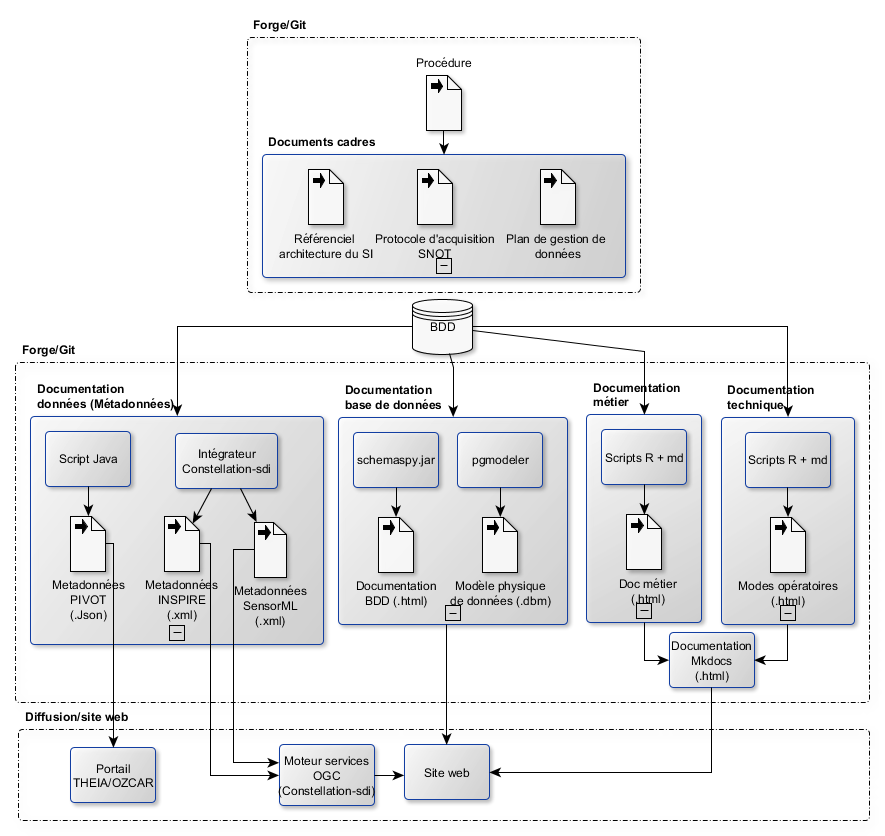
\includegraphics[width=14cm]{Diagramme_documentation.png}
		\caption{Procédure globale pour la génération de la documentation du SI \SNOT}
		\label{Procedure_documentation}		
	\end{center}
\end{figure}

\subsection{Les documents cadres}

Dans cette partie, développer rapidement et renvoyer vers les liens de consultation des documents cadres du projet. Expliquer brièvement l'intérêt d'avoir ce type de document et leur philosophie de document évolutif...

\subsubsection{Référentiel architecture du SI}

\subsubsection{Protocole d'acquisition}

\subsubsection{Plan de gestion de données}





\subsection{Documentation des données et des instruments : les métadonnées}

La documentation des données et des instruments du \SNOT est organisée par jeu de données et sous la forme de plusieurs types de métadonnées standardisées.

\subsubsection{Organisation par jeu de données}
% Voir si création des métadonnées par jeu de données ou par type de jeu de données
Pour faciliter la création des métadonnées du \SNOT, il a été décidé de générer des métadonnées au niveau des jeux de données. Les jeux de données correspondent aux données collectées sur les sites du \SNOT couvrant une même thématique. Le \SNOT couvre 5 jeux de données :

	\begin{itemize}
		\item Biogéo : Ensemble des données d'origine biogéochimique de l'eau,
		\item Bioveg : Ensemble des données liées à la biodiversité et à la végétation,
		\item GES : Ensemble des données associées à la collecte des Gaz à Effet de Serrre (GES),
		\item Hydro-Carto : Données hydrologiques des sites du \SNOT,
		\item Météo-sol : Données météorologiques et physiques du sol.
	\end{itemize}

\subsubsection{Les métadonnées OZCAR/PIVOT}

\subsubsection{Les métadonnées standardisées OGC}

\subsection{Documentation de la base de données}

La base de données du SI \SNOT représente le système où les données collectées sur les sites du \SNOT sont organisées afin de faciliter leur compréhension, leur diffusion/extraction et leur maintenance. La documentation de l'organisation des données et de son contenu dans la base est donc très important. Cette documentation est basée sur deux outils.

\subsubsection{Présentation de la base de données}

La documentation est générée automatiquement avec le programme \mhref{http://schemaspy.org/}{schemaspy.jar}. Ce programme permet de générer un site web statique en se connectant à une base de données. L'utilisateur peut ainsi visualiser dans le détail l'organisation des tables et leur contenus. Le mode opératoire suivant permet d'utiliser ce programme : %RAjouter l'adresse du mode opératoire.

\subsubsection{Les modèles physiques de données}

Les modèles physiques de données de la base de données sont générés avec le logiciel \mhref{https://pgmodeler.io/}{pgmodeler}. Pour plus de détails sur la construction de ces modèles, consultez le mode opératoire suivant : %RAjouter l'adresse du mode opératoire.

\subsection{Documentation métier}

Une documentation métier est générée pour expliquer le cycle de vie de chaque type du jeu de données du \SNOT (Biogéo, Bioveg, GES, Hydro-Carto, Météo-sol). La création de cette documentation est expliquée dans le mode opératoire suivant. %RAjouter l'adresse du mode opératoire
\mhref{\adressedocsmetier/Sce_modele.html}{Un modèle de scénario d'échange} est ainsi proposé.
Il est consultable également sur la documentation générale du \SNOT.
Cette documentation prend la forme de deux type de documents :
\begin{itemize}
	\item \texttt{Sce\_jeudedonnées.html} : Les scénarios d'échanges (\texttt{Sce}) pour chaque type de jeu de données. Ce document décrit les modalités d'échange des fichiers issues de la collecte de chaque type de jeu de données (format, règle de nommage des fichiers \dots)
	\item \texttt{Bdd\_jeudedonnées.html} : Un document présentant la modélisation de chaque type de jeu de données est également créé.
\end{itemize}

\subsection{Documentation technique}

Toute la documentation technique est proposée sous la forme de mode opératoire. Ces modes opératoires sont consultables à cette adresse. Un mode opératoire décrit comment créer ou mettre à jour ces fichiers.




\end{document}
